\documentclass{article}

% Copy/pasta of nips_2017 for future modification found here:
% https://nips.cc/Conferences/2017/PaperInformation/StyleFiles


% if you need to pass options to natbib, use, e.g.:
% \PassOptionsToPackage{numbers, compress}{natbib}
% before loading nips_2017
%
% to avoid loading the natbib package, add option nonatbib:
% \usepackage[nonatbib]{nips_2017}

\usepackage{nips_2017}

% to compile a camera-ready version, add the [final] option, e.g.:
% \usepackage[final]{nips_2017}

\usepackage[utf8]{inputenc} % allow utf-8 input
\usepackage[T1]{fontenc}    % use 8-bit T1 fonts
\usepackage{hyperref}       % hyperlinks
\usepackage{url}            % simple URL typesetting
\usepackage{booktabs}       % professional-quality tables
\usepackage{amsfonts}       % blackboard math symbols
\usepackage{nicefrac}       % compact symbols for 1/2, etc.
\usepackage{microtype}      % microtypography
\usepackage{pdfpages}       % Because LaTeX doesn't take SVGs...
\usepackage{amsmath}
\usepackage{algorithm}
\usepackage{algorithmic}
\usepackage{natbib}


\title{Pulsar Classification using Deep Neural Networks}

\author{
  Kyle W.~MacMillan
  Department of Computer Science\\
  South Dakota School of Mines and Technology\\
  Rapid City, SD 57701 \\
  \texttt{kyle.macmillan@mines.sdsmt.edu} \\
}

\begin{document}

\maketitle

\begin{abstract}
  Pulsars are rapidly rotating, highly magnetized, neutron stars and white 
  dwarfs that emit focused electromagnetic radiation in a beam. The beam is 
  only visible to us when it is directly facing Earth and is the reason for 
  their pulsed nature. This paper approaches classification of pulsars and 
  non-pulsars with the intent of learning more about TensorFlow. The 
  classification method used is Deep Neural Networks and an acceptable level of 
  accuracy was obtained.
\end{abstract}

\section{Introduction}
  We were tasked with picking a dataset and training a deep learning network. 
  First thing to do was to pick a dataset. Being an open-ended assignment there 
  was uncertainty as to what particular dataset to explore. Initial looks 
  involved different image classification datasets such as CIFAR-10, 
  Caltech 101, and NORB. Down the road there is no desire to work with image 
  data classification, work with files and datasets of continuous and 
  discrete data are preferred. After thorough search of the available datasets 
  it was decided pulsar classification best suited this paper. 

  The last decision before pressing on to data format was to pick the correct 
  deep learning framework for the job. There were several options but 
  TensorFlow seemed like a good choice. Keras and PyTorch are other tools that 
  utilize TensorFlow but were not used because those are often considered a 
  "front end" for TensorFlow, which was not part of the goals of the 
  assignment.

\section{Method}

\subsection{Main}
  Main.py is where the project is ran from. There are several hyperparameters 
  that a user can pick, beginning with $\_TEST\_PERCENTAGE$, which sets the 
  percentage of comma-separated values (CSV) data to be utilized for testing. 
  Industry standard is 20\%, so that is the default setting. The training data 
  $\_TRAIN$ is, as a result, 80\% of the CSV data. 
  % 
  \[\mathcal{\_TRAIN}=\_NUM\_ELEMENTS * ( 1 - \_TEST\_PERCENTAGE )\]
  % 
  It was necessary to hard-code in the number of elements in the CSV file because there was trouble when trying to run update on the CSV class due to 
  an incomplete understanding of python abilities such as $class.update()$.

  $\_BATCH\_SIZE$ is set as 
  %
  \[\mathcal{\_BATCH\_SIZE}=max\{\_TRAIN*0.1, 1\}\]
  %
  This is part of ensuring the training does not get stuck in local minima. \_MODEL is then set as whichever optimizer the user would like, in this case, 
  RMSPropOptimizer was selected. A CSV class is created based on the dataset to 
  be classified. 

  Hyperparameter choices are part of the art of machine learning but in this 
  project it was not the focus to make perfect hyperparameters. That being 
  said, that was explored briefly for this project as seen in section 
  \ref{sec:hyperparams}. $\_NODES\_PER\_LAYER$ was one of such hyperparameters, 
  as was $\_LAYERS$, and $\_HIDDEN\_LAYERS$. The final implementation of these 
  parameters are as follows:
  %
  \[\mathcal{\_NODES\_PER\_LAYER}=(num\_features - 1) * 1.5\]
  \[\mathcal{\_LAYERS}=max\{sqrt(\_NODES\_PER\_LAYER), 2\}\]
  \[\mathcal{\_HIDDEN\_LAYERS}=[\_NODES\_PER\_LAYER] * \_LAYERS\]
  %
  This lead to 3 hidden layers with 12 nodes each for the \href{https://archive.ics.uci.edu/ml/datasets/HTRU2}{HTRU\_2 Dataset}.

  After all parameters have been setup main gets run. Users can select the 
  number of runs to perform as an argument when they begin the program e.g. 
  %
  \[\textnormal{python\ main.py \textit{X}}\]  
  %
  The program will then run the classifier \textit{X} times. After finishing 
  the program will output classification accuracy of the given dataset.



\subsection{Data format}
  After determining the dataset and the framework to be utilized it is 
  necessary to figure out how to read data from the dataset. A modular approach 
  was taken with this project. Users will be able to select a CSV file to load 
  in. By specifying a class to contain the CSV data it is possible to run 
  multiple datasets while making only minor modifications to the code. The 
  format is also much easier to read as a result of the class format.

  Rather than code up a custom method of moving CSV data into a format usable 
  by the deep learning framework it was determined to "stand on the shoulders 
  of giants". Pandas was used to bring CSV data into usable form. After pulling 
  the data into a single structure it was necessary to split the data into 
  training and testing data. Again, rather than code that from scratch it was 
  determined best practice to utilize existing tools. 

  For that endevour scikit-learn was used, specifically the 
  $train\_test\_split()$ method. As is standard for classification problems the 
  data was segmented into 80\% training and 20\% testing data. It was then 
  necessary to place the $class$ label into a data structure for later. For 
  both the train and test data, associated labels are passed, along with the 
  data, as tuples. The psuedocode for this section can be found under Algorithm 
  \ref{alg:input_fn}.
  %
  \begin{algorithm}
    \caption{$input\_fn()$}
    \label{alg:input_fn}
    \begin{algorithmic}
      \STATE $data \gets CSV$\\
      \STATE $test, train \gets train\_test\_split(data)$
      \STATE $test\_label \gets test.pop(class)$
      \STATE $train\_label \gets train.pop(class)$
      \RETURN $(train, train\_label), (test,test\_label)$
    \end{algorithmic}
  \end{algorithm}
  %
\subsection{TensorFlow estimator}
  TensorFlow has built in estimators such as:
  %
  \begin{itemize}
    \item \href{https://www.tensorflow.org/api_docs/python/tf/estimator/DNNClassifier}{DNNClassifier}
    \item \href{https://www.tensorflow.org/api_docs/python/tf/estimator/BaselineClassifier}{BaselineClassifier}
    \item \href{https://www.tensorflow.org/api_docs/python/tf/estimator/BaselineRegressor}{BaselineRegressor}
    \item \href{https://www.tensorflow.org/api_docs/python/tf/estimator/DNNLinearCombinedClassifier}{DNNLinearCombinedClassifier}
    \item \href{https://www.tensorflow.org/api_docs/python/tf/estimator/LinearClassifier}{LinearClassifier}
    \item \href{https://www.tensorflow.org/api_docs/python/tf/estimator/LinearRegressor}{LinearRegressor}
  \end{itemize}
  %
  You also have the ability to build your own estimator, or classifier, and 
  this is the route that was selected for this project. The custom estimator 
  selected utilizes the $model$ specified at the start of the program, a 
  $model\_dir$ for TensorBoard output which will be discussed in section 
  \ref{sec:tensorboard}, and the $params$ which consist of $feature\_columns$, 
  $hidden\_units$, and $n\_classes$.

  Estimator also requires \href{https://www.tensorflow.org/versions/r1.2/api_docs/python/tf/estimator/ModeKeys}{three modes} depending on the goal:
  %
  \begin{itemize}
    \item ModeKeys.TRAIN
    \item ModeKeys.EVAL
    \item ModeKeys.PREDICT
  \end{itemize}
  %
  Lastly, the estimator requires a return of $EstimatorSpec$. Documentation for 
  the EstimatorSpec can be found on \href{https://www.tensorflow.org/api_docs/python/tf/estimator/EstimatorSpec}{TensorFlow's website}. It is important to note that each of the different $ModeKeys$ requires a different set of parameters for the returned $EstimatorSpec$.

\subsection{Training}
  TensorFlow offers the ability to train estimators by calling a $train()$ 
  method. For this paper the $input\_fn$ and $steps$ arguments are set by a 
  function call to $train\_input\_fn$ and $csv.num\_examples['train']$ 
  respectively. This allows the data to be segmented for training.

  The model that was instantiated during estimator creation is detailed under
  $\textnormal{model.model\_RMSProp}$. For each of the layers that was passed 
  to it under $params['hidden\_units']$ there is a fully connected layer built 
  with selu activation. \citet{selu} found with the proper math you can obtain 
  self-normalizing exponential linear units, meaning they don't require batch 
  normalization and that is why they were chosen over all of the other 
  activation functions. There is also the final fully connected layer which has 
  no activation layer. This final layer aids in determining the classification.

  During training ModeKeys.TRAIN is called, which specifies RMSProp gradient 
  descent as our optimizer and then calls $minimize()$. The $minimize()$ method 
  will automatically compute the gradients and apply them to the variables, but 
  if you need to tune the network there are additional steps that can be taken 
  instead:
  %
  \begin{enumerate}
    \item Compute the gradients with $compute\_gradients()$
    \item Process the gradients as you wish
    \item Apply the processed gradients with $apply\_gradients()$
  \end{enumerate}
  %
  Further documentation on this process can be found on TensorFlow's website 
  under the \href{https://www.tensorflow.org/api_docs/python/tf/train/Optimizer}
  {class Optimizer}. It was not necessary to have that level of fidelity with 
  this particular dataset, so the base $minimize()$ was all that was necessary.

  With $minimize()$ minimizing the loss we are able to make progress towards a 
  classification. This dataset in particular minimizes loss to near-zero after 
  just the first episode of 100 training steps as can be seen in Figure \ref{img:loss}.


\subsection{Hyperparameters}\label{sec:hyperparams}
  Hyperparameters are normally very important but in this dataset it was 
  discovered that they had very little impact on the efficacy of 
  this classifier.

  An example of hyperparameter randomization can be found under:
  %
  \[\textnormal{python\ hyperparams.py}\]
  %
  That file will automatically generate randomized hyperparameters. During 
  testing of this project various hyperparameters were tested with no 
  significant improvements over the initial parameters set so the associated 
  code was removed from primary operation of the classifier. The file described 
  would allow for random testing of hyperparameters across any number of 
  computers. \citet{hypparam} found random search of hyperparameters to be superior to grid search and was the method used while exploring 
  hyperparameter tuning during this project.

\subsection{TensorBoard}\label{sec:tensorboard}
  One of the other reasons for utilizing TensorFlow is the TensorBoard project. 
  TensorBoard allows for visualization of various parameters as defined by the 
  user. Figure \ref{img:acc_smooth} and \ref{img:loss_smooth} are the same results as shown in Figure \ref{img:accuracy} and \ref{img:loss} 
  respectively. The smooothing helps in understanding what may be going on, 
  especially in more turbulant graphs. Another benefit is being able to 
  visualize the graph structure. To use TensorBoard on this project ensure it 
  was installed with TensorFlow and type 
  \[\textnormal{tensorboard\ -\--logdir\ model}\]
  and go to the link it provides (by ctrl clicking or copy/paste). 

  \begin{figure}[H]
  \caption{Smoothed Accuracy}\label{img:acc_smooth}
  \begin{center}
  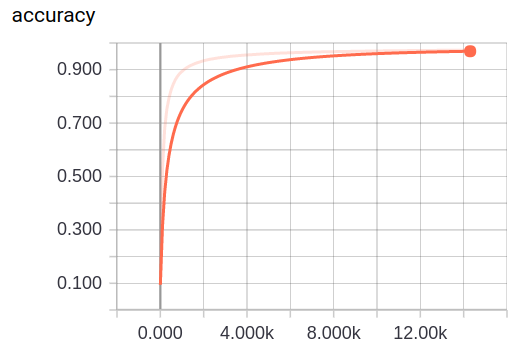
\includegraphics[scale=0.65]{../images/acc}
  \end{center}
  \end{figure}
  %
  \begin{figure}[H]
  \caption{Smoothed Loss}\label{img:loss_smooth}
  \begin{center}
  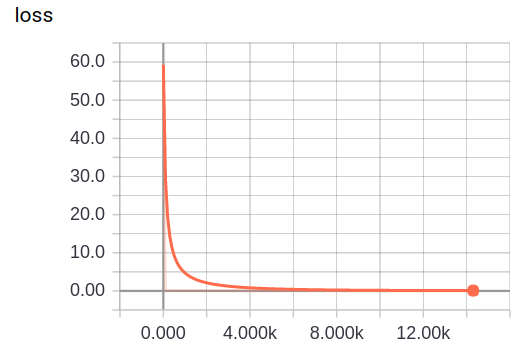
\includegraphics[scale=0.65]{../images/loss}
  \end{center}
  \end{figure}




\newpage
\section{Results}\label{sec:results}
  RMSProp gradient descent with 0.001 learning rate, performing batch runs on 
  10\% of the training samples every 100 steps produced an accuracy of 97.8\% 
  averaged over 20 tests. These were taken with 80\% train and 20\% test 
  samples. Other hyperparameters were three fully connected layers with 12 
  nodes each using selu activation. 

  \begin{figure}[H]
  \caption{Accuracy}\label{img:term_acc}
  \begin{center}
  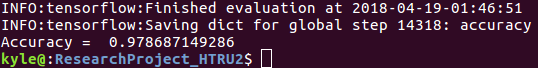
\includegraphics[scale=0.75]{../images/accuracy_percent_small}
  \end{center}
  \end{figure}
  %
  \begin{figure}[H]
  \caption{Accuracy}\label{img:accuracy}
  \begin{center}
  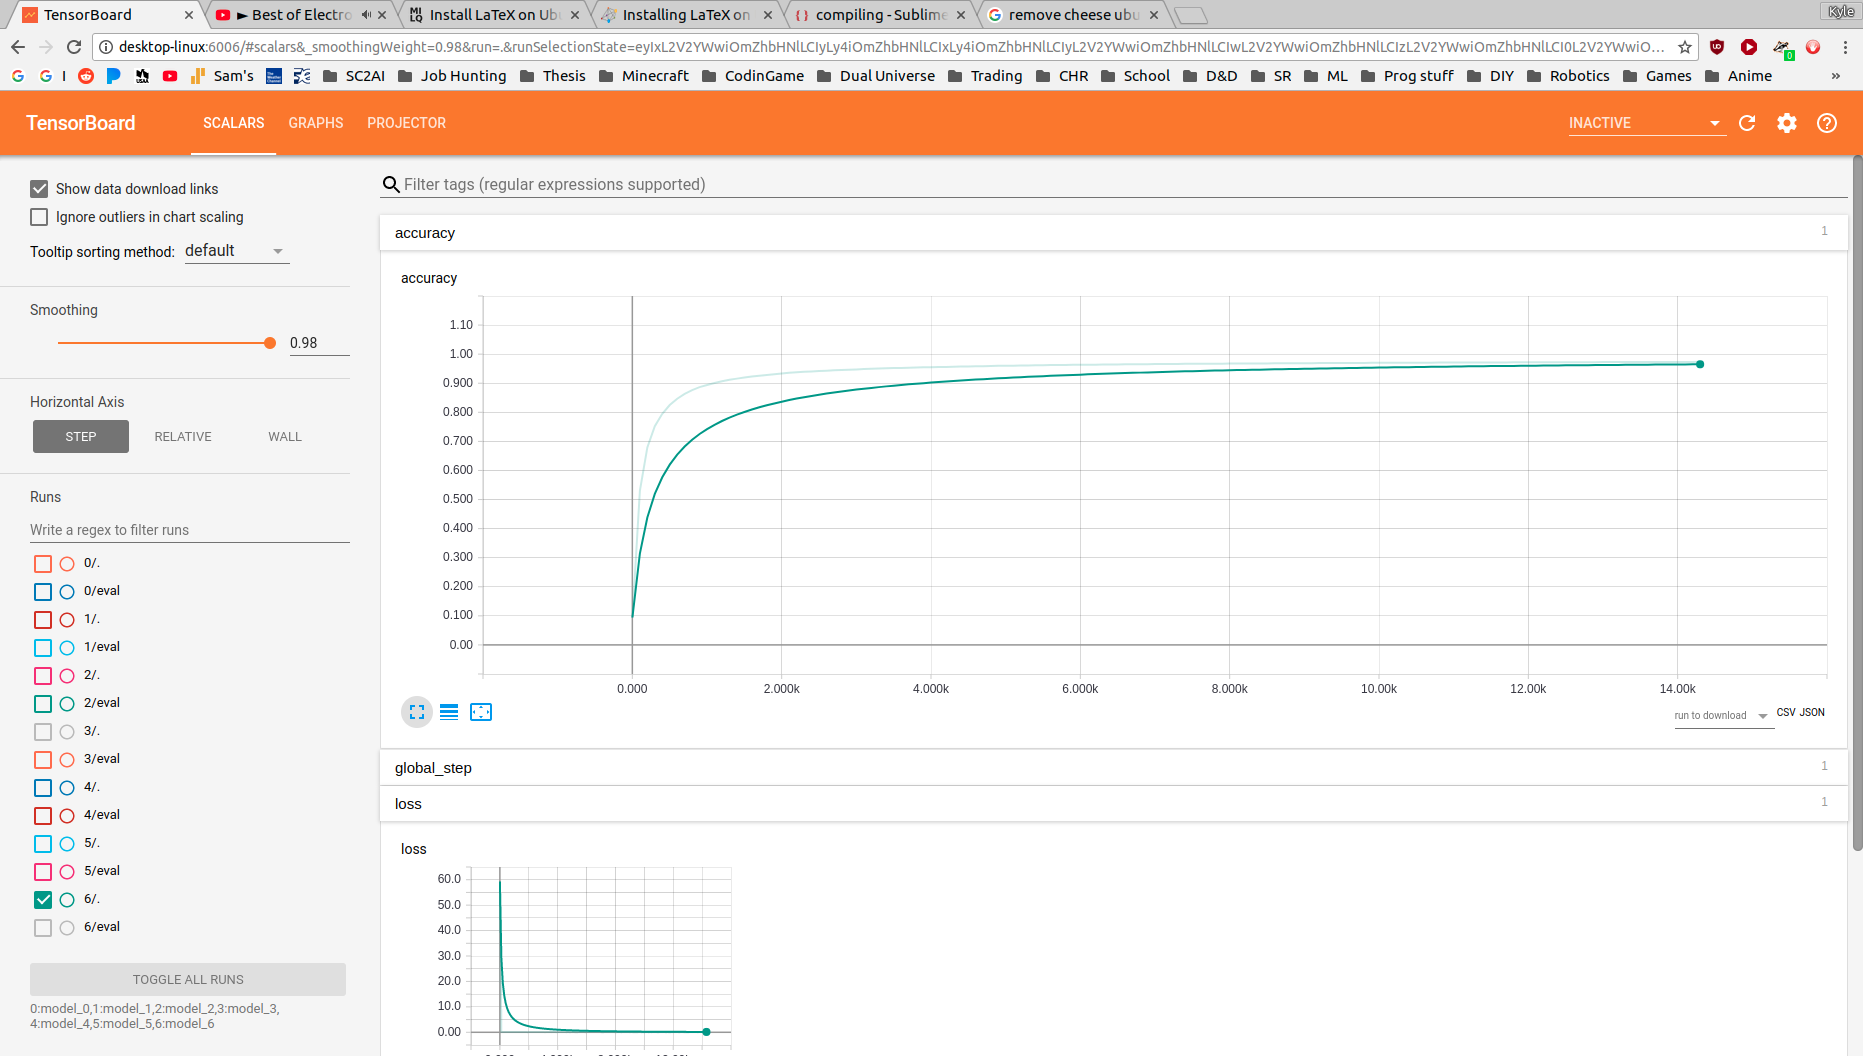
\includegraphics[scale=0.75]{../images/Accuracy}
  \end{center}
  \end{figure}
  %
  \begin{figure}[H]
  \caption{Loss}\label{img:loss}
  \begin{center}
  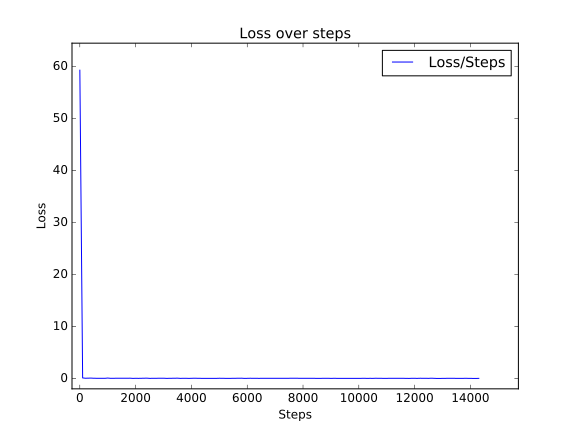
\includegraphics[scale=0.75]{../images/Loss}
  \end{center}
  \end{figure}

\section{Conclusion}




\section{General formatting instructions}
\label{gen_inst}

The text must be confined within a rectangle 5.5~inches (33~picas)
wide and 9~inches (54~picas) long. The left margin is 1.5~inch
(9~picas).  Use 10~point type with a vertical spacing (leading) of
11~points.  Times New Roman is the preferred typeface throughout, and
will be selected for you by default.  Paragraphs are separated by
\nicefrac{1}{2}~line space (5.5 points), with no indentation.

The paper title should be 17~point, initial caps/lower case, bold,
centered between two horizontal rules. The top rule should be 4~points
thick and the bottom rule should be 1~point thick. Allow
\nicefrac{1}{4}~inch space above and below the title to rules. All
pages should start at 1~inch (6~picas) from the top of the page.

For the final version, authors' names are set in boldface, and each
name is centered above the corresponding address. The lead author's
name is to be listed first (left-most), and the co-authors' names (if
different address) are set to follow. If there is only one co-author,
list both author and co-author side by side.

Please pay special attention to the instructions in Section \ref{others}
regarding figures, tables, acknowledgments, and references.

\section{Headings: first level}
\label{headings}

All headings should be lower case (except for first word and proper
nouns), flush left, and bold.

First-level headings should be in 12-point type.

\subsection{Headings: second level}

Second-level headings should be in 10-point type.

\subsubsection{Headings: third level}

Third-level headings should be in 10-point type.

\paragraph{Paragraphs}

There is also a \verb+\paragraph+ command available, which sets the
heading in bold, flush left, and inline with the text, with the
heading followed by 1\,em of space.

\section{Citations, figures, tables, references}
\label{others}

These instructions apply to everyone.

\subsection{Citations within the text}

The \verb+natbib+ package will be loaded for you by default.
Citations may be author/year or numeric, as long as you maintain
internal consistency.  As to the format of the references themselves,
any style is acceptable as long as it is used consistently.

The documentation for \verb+natbib+ may be found at
\begin{center}
  \url{http://mirrors.ctan.org/macros/latex/contrib/natbib/natnotes.pdf}
\end{center}
Of note is the command \verb+\citet+, which produces citations
appropriate for use in inline text.  For example,
\begin{verbatim}
   \citet{hasselmo} investigated\dots
\end{verbatim}
produces
\begin{quote}
  Hasselmo, et al.\ (1995) investigated\dots
\end{quote}

If you wish to load the \verb+natbib+ package with options, you may
add the following before loading the \verb+nips_2017+ package:
\begin{verbatim}
   \PassOptionsToPackage{options}{natbib}
\end{verbatim}

If \verb+natbib+ clashes with another package you load, you can add
the optional argument \verb+nonatbib+ when loading the style file:
\begin{verbatim}
   \usepackage[nonatbib]{nips_2017}
\end{verbatim}

As submission is double blind, refer to your own published work in the
third person. That is, use ``In the previous work of Jones et
al.\ [4],'' not ``In our previous work [4].'' If you cite your other
papers that are not widely available (e.g., a journal paper under
review), use anonymous author names in the citation, e.g., an author
of the form ``A.\ Anonymous.''

\subsection{Footnotes}

Footnotes should be used sparingly.  If you do require a footnote,
indicate footnotes with a number\footnote{Sample of the first
  footnote.} in the text. Place the footnotes at the bottom of the
page on which they appear.  Precede the footnote with a horizontal
rule of 2~inches (12~picas).

Note that footnotes are properly typeset \emph{after} punctuation
marks.\footnote{As in this example.}

\subsection{Figures}

All artwork must be neat, clean, and legible. Lines should be dark
enough for purposes of reproduction. The figure number and caption
always appear after the figure. Place one line space before the figure
caption and one line space after the figure. The figure caption should
be lower case (except for first word and proper nouns); figures are
numbered consecutively.

You may use color figures.  However, it is best for the figure
captions and the paper body to be legible if the paper is printed in
either black/white or in color.
\begin{figure}[h]
  \centering
  \fbox{\rule[-.5cm]{0cm}{4cm} \rule[-.5cm]{4cm}{0cm}}
  \caption{Sample figure caption.}
\end{figure}

\subsection{Tables}

All tables must be centered, neat, clean and legible.  The table
number and title always appear before the table.  See
Table~\ref{sample-table}.

Place one line space before the table title, one line space after the
table title, and one line space after the table. The table title must
be lower case (except for first word and proper nouns); tables are
numbered consecutively.

Note that publication-quality tables \emph{do not contain vertical
  rules.} We strongly suggest the use of the \verb+booktabs+ package,
which allows for typesetting high-quality, professional tables:
\begin{center}
  \url{https://www.ctan.org/pkg/booktabs}
\end{center}
This package was used to typeset Table~\ref{sample-table}.

\begin{table}[t]
  \caption{Sample table title}
  \label{sample-table}
  \centering
  \begin{tabular}{lll}
    \toprule
    \multicolumn{2}{c}{Part}                   \\
    \cmidrule{1-2}
    Name     & Description     & Size ($\mu$m) \\
    \midrule
    Dendrite & Input terminal  & $\sim$100     \\
    Axon     & Output terminal & $\sim$10      \\
    Soma     & Cell body       & up to $10^6$  \\
    \bottomrule
  \end{tabular}
\end{table}

\section{Final instructions}

Do not change any aspects of the formatting parameters in the style
files.  In particular, do not modify the width or length of the
rectangle the text should fit into, and do not change font sizes
(except perhaps in the \textbf{References} section; see below). Please
note that pages should be numbered.

\section{Preparing PDF files}

Please prepare submission files with paper size ``US Letter,'' and
not, for example, ``A4.''

Fonts were the main cause of problems in the past years. Your PDF file
must only contain Type 1 or Embedded TrueType fonts. Here are a few
instructions to achieve this.

\begin{itemize}

\item You should directly generate PDF files using \verb+pdflatex+.

\item You can check which fonts a PDF files uses.  In Acrobat Reader,
  select the menu Files$>$Document Properties$>$Fonts and select Show
  All Fonts. You can also use the program \verb+pdffonts+ which comes
  with \verb+xpdf+ and is available out-of-the-box on most Linux
  machines.

\item The IEEE has recommendations for generating PDF files whose
  fonts are also acceptable for NIPS. Please see
  \url{http://www.emfield.org/icuwb2010/downloads/IEEE-PDF-SpecV32.pdf}

\item \verb+xfig+ "patterned" shapes are implemented with bitmap
  fonts.  Use "solid" shapes instead.

\item The \verb+\bbold+ package almost always uses bitmap fonts.  You
  should use the equivalent AMS Fonts:
\begin{verbatim}
   \usepackage{amsfonts}
\end{verbatim}
followed by, e.g., \verb+\mathbb{R}+, \verb+\mathbb{N}+, or
\verb+\mathbb{C}+ for $\mathbb{R}$, $\mathbb{N}$ or $\mathbb{C}$.  You
can also use the following workaround for reals, natural and complex:
\begin{verbatim}
   \newcommand{\RR}{I\!\!R} %real numbers
   \newcommand{\Nat}{I\!\!N} %natural numbers
   \newcommand{\CC}{I\!\!\!\!C} %complex numbers
\end{verbatim}
Note that \verb+amsfonts+ is automatically loaded by the
\verb+amssymb+ package.

\end{itemize}

If your file contains type 3 fonts or non embedded TrueType fonts, we
will ask you to fix it.

\subsection{Margins in \LaTeX{}}

Most of the margin problems come from figures positioned by hand using
\verb+\special+ or other commands. We suggest using the command
\verb+\includegraphics+ from the \verb+graphicx+ package. Always
specify the figure width as a multiple of the line width as in the
example below:
\begin{verbatim}
   \usepackage[pdftex]{graphicx} ...
   \includegraphics[width=0.8\linewidth]{myfile.pdf}
\end{verbatim}
See Section 4.4 in the graphics bundle documentation
(\url{http://mirrors.ctan.org/macros/latex/required/graphics/grfguide.pdf})

A number of width problems arise when \LaTeX{} cannot properly
hyphenate a line. Please give LaTeX hyphenation hints using the
\verb+\-+ command when necessary.

\subsubsection*{Acknowledgments}

Use unnumbered third level headings for the acknowledgments. All
acknowledgments go at the end of the paper. Do not include
acknowledgments in the anonymized submission, only in the final paper.

\section*{References}

References follow the acknowledgments. Use unnumbered first-level
heading for the references. Any choice of citation style is acceptable
as long as you are consistent. It is permissible to reduce the font
size to \verb+small+ (9 point) when listing the references. {\bf
  Remember that you can go over 8 pages as long as the subsequent ones contain
  \emph{only} cited references.}
\medskip

\small

[1] Alexander, J.A.\ \& Mozer, M.C.\ (1995) Template-based algorithms
for connectionist rule extraction. In G.\ Tesauro, D.S.\ Touretzky and
T.K.\ Leen (eds.), {\it Advances in Neural Information Processing
  Systems 7}, pp.\ 609--616. Cambridge, MA: MIT Press.

[2] Bower, J.M.\ \& Beeman, D.\ (1995) {\it The Book of GENESIS:
  Exploring Realistic Neural Models with the GEneral NEural SImulation
  System.}  New York: TELOS/Springer--Verlag.

[3] Hasselmo, M.E., Schnell, E.\ \& Barkai, E.\ (1995) Dynamics of
learning and recall at excitatory recurrent synapses and cholinergic
modulation in rat hippocampal region CA3. {\it Journal of
  Neuroscience} {\bf 15}(7):5249-5262.

% [4] Bergstra, J.\ \& Bengio, J.\ (2012) Random Search for Hyper-Parameter 
% Optimization. {\it Journal of Machine Learning Research 13} pp.\ 281-305.

\bibliographystyle{plainnat}
\bibliography{bib}
\end{document}